\chapter{The Mindset Behind an Unforgettable Novel}

This lecture is an interview rather than a blackboard lecture, so its rigor is not symbolic in the usual sense. It is procedural, comparative, and architectural. The opening half-minute functions as an overture: we hear, before the conversation properly begins, the lecture's eventual claims about readerly presence, outlining, poetic surprise, and the iterative feedback loop of description. Then the discussion resets and begins where the host actually begins, with admiration for Amor Towles's descriptive precision and vocabulary. What follows is a systematic account of fictional craft: how language evokes a social world, how description produces presence, how planning frees surprise, how point of view generates symbolism, and how revision converts private fascination into a form worthy of the reader's time. This conversation between David Perell and Amor Towles belongs to the curated LazyingArt LLC collection \emph{How You Speak and Write}.

\section{Prelude, Vocabularies, and Social Worlds}

The first real movement of the lecture begins not with plot, pacing, or symbolism, but with vocabulary. Perell notices Towles's ease with socially precise language, and in particular with French-inflected diction in \emph{A Gentleman in Moscow}. Towles's answer is immediately broader than the prompt. A writer, he says, becomes interested in many vocabularies: baseball, city streets, finance, ethnicity, technical disciplines, even the language of physics. The point is not accumulation for its own sake. The point is that different situations ask for different lexical pressures, and a writer gradually learns to hear those pressures.

This is why Towles's example of the Count matters. Count Rostov is an aristocrat formed in late nineteenth-century Europe. French is therefore not a decorative garnish; it belongs to the atmosphere of his world. Towles makes the point more sharply by admitting that he himself does not speak French fluently. What he wants is not philological completeness, but the right evocation. A few carefully placed elements can help bring into focus the kind of person this is, and the kind of culture that formed him.

From there the discussion broadens to a second contrast. If \emph{A Gentleman in Moscow} draws on aristocratic and European registers, \emph{The Lincoln Highway} must sound like midcentury America. To prepare that soundscape, Towles revisits several American books written around the same historical moment. The exact bibliographic sequence in the transcript is somewhat unstable, but the underlying argument is clear: books published within roughly the same period can still carry radically different vocabularies, thematic concerns, and social tonalities, while remaining unmistakably American. Language is therefore not merely a sign of verbal skill. It is a way of choosing a world.

\subsection{Question \& Answer}

\paragraph{How do we use a language-world that we only partly possess ourselves?}

Towles's answer is practical and modest. We do not wait for total mastery. We listen, absorb, and gather fragments that carry real social pressure. Then, when we write, we draw on what we have heard in order to evoke sensibility rather than to display credentials. The standard is not that we become encyclopedic masters of every register. The standard is that the chosen language belongs to the world of the character, the class, the profession, or the historical situation.

\section{Readerly Presence and the Economy of Description}

Perell's transition into Towles's essay on Hopper's \emph{Nighthawks} shifts the discussion from vocabulary to effect. He describes the experience of encountering a mood he had not previously named. Towles responds by identifying the deeper aim. The most important thing, he says, is to make the reader feel as though they are living the experience in the book. Description matters because it is one of the chief means by which that state is achieved.

\begin{definition}
By \emph{readerly presence} we mean the condition in which the reader feels located inside the scene, can orient himself within it, and can therefore become interested in the unfolding thoughts, feelings, and actions of the characters.
\end{definition}

Towles's causal chain is explicit enough that we may safely render it schematically:
\begin{equation}
\text{description} \longrightarrow \text{readerly presence} \longrightarrow \text{readerly engagement}.
\end{equation}
This is not lecture-board mathematics. It is a compact notation for a spoken argument. Description is valuable because it lets the reader feel present, and presence is what allows the reader to become connected to character and event.

The hotel in \emph{A Gentleman in Moscow} supplies the model case. Because the novel remains inside that environment for decades, Towles knows that the geography of the hotel must be laid out early. Key rooms must become vivid early. If that initial orientation is successful, later movement through the building will feel natural rather than arbitrary.

A second relation follows from this:
\begin{align}
\text{too little detail} &\Rightarrow \text{weak presence}, \\
\text{too much detail} &\Rightarrow \text{drag}, \\
\text{effective description} &\text{ lies in the narrow middle region.}
\end{align}
The local transcript is noisy at precisely this point, but the underlying claim is unambiguous. Description cannot be so spare that the scene could be anywhere, and it cannot be so specific and cumbersome that the reader becomes trapped in cold inventory. The writer adds details, removes details, and narrows in on the few elements that make the space come alive.

\begin{figure}[h]
\centering
\begin{tikzpicture}[>=stealth]
\node[draw, rectangle, minimum width=3.0cm, minimum height=0.9cm] (a) at (0,0) {Describe};
\node[draw, rectangle, minimum width=3.0cm, minimum height=0.9cm] (b) at (4.2,0) {See More};
\node[draw, rectangle, minimum width=3.6cm, minimum height=0.9cm] (c) at (8.8,0) {Describe More};
\draw[->] (a) -- (b);
\draw[->] (b) -- (c);
\draw[->] (c) to[out=35,in=145] (a);
\end{tikzpicture}
\caption{Transcript-based schematic reconstruction of Towles's iterative loop. Description sharpens perception, and sharpened perception returns to language.}
\end{figure}

The overture at the very beginning of the lecture gave this loop in compressed form, and later Towles states it directly:
\begin{equation}
\text{describe} \longrightarrow \text{see more} \longrightarrow \text{describe more}.
\end{equation}
The important point is that description is not merely report. Once we begin to describe, we begin to notice more, and what we notice more deeply becomes available for further description.

\subsection{Question \& Answer}

\paragraph{How much description is enough to make a place vivid without bogging the reader down?}

Enough to orient the reader, not enough to imprison him. The writer does not aim at exhaustive totality. He aims at the set of details that will let the reader know where he is, move through the room, and feel events taking place there. In practice this means writing, rereading, adding, subtracting, and discovering which details are actually doing the work.

\section{Pacing, Editing, and Urgency Without Action}

From the balance of description the lecture naturally turns to tempo. Perell asks the right question: how do we judge pacing when repeated exposure distorts our own sense of it? Towles answers by renaming the subject. What Perell is really asking about, he says, is editing.

Writing and editing are closely interlinked but not identical. Editing is the effort to return to what one has already written and hear it with a colder ear. Towles gives a simple but severe criterion: if a passage feels boring to him on rereading, that is already a warning sign. The reader is even more at risk.

The key clarification is that pace is not the same as page-turning action. Towles explicitly refuses that reduction:
\begin{equation}
\text{urgency} \neq \text{action}.
\end{equation}
A classical page-turner is driven by external crisis, danger, and event. That is one art form. Literary urgency is broader. A reader may be drawn forward by curiosity about a character's psychology, by tonal pressure, by a sentence whose phrasing compels the next sentence, or by the sheer wish to understand how a mind will respond, even when outward action is minimal.

This distinction matters because it preserves a freedom that many discussions of pacing destroy. A literary novel may contain slow passages. What matters is whether the slowness is alive. If the prose continues to generate inward motion, then the reader is still being carried.

\subsection{Question \& Answer}

\paragraph{How can a novel create urgency when little external action is occurring?}

By making continuation necessary. The reader can be compelled forward by a character's consciousness, by phrasing, by emotional tension, by tonal suspense, or by the pressure of a question that has not yet been answered. This is why Towles insists that the aim is not simply speed. It is momentum.

\section{Premise, Scaffolding, and Freeing the Poetic Mind}

After the discussion of pacing, Towles steps back and describes the architecture of his process. This is one of the lecture's most formal passages. His novels begin, he says, with a very simple premise: one compressed sentence, something like a man trapped in a hotel for a long period of time. If the premise has force, it expands rapidly. In the case of \emph{A Gentleman in Moscow}, the setting, social identity, historical frame, and central constraints appear almost immediately.

We can summarize the pipeline as follows:
\begin{equation}
\text{premise} \longrightarrow \text{scaffolding} \longrightarrow \text{notebooks} \longrightarrow \text{draft} \longrightarrow \text{revision}.
\end{equation}

Towles is unusually concrete about timing:
\begin{enumerate}
\item In about \(1.5\) hours, he wrote down the key elements of \emph{A Gentleman in Moscow}.
\item Over roughly \(3\) days, he wrote the scaffolding for most of the key events.
\item Over a couple of years, he filled notebooks with scene investigations, questions, and visualized moments.
\item Only then did he write the book itself, over about \(1.5\) years.
\item After that came \(2\) or \(3\) revision passes from beginning to end.
\end{enumerate}

The notebooks matter because they remove live uncertainty from the drafting stage. Towles is not sitting before a blank page trying to decide where the room is, who is present, what the emotional context is, and what event should occur. Those decisions have largely been precomputed. The actual drafting question becomes a better one: what is the best language for bringing this already imagined scene to life?

This leads to the lecture's most memorable process equation:
\begin{equation}
\text{more precomputed structure} \Rightarrow \text{less analytic load} \Rightarrow \text{more poetic freedom}.
\end{equation}
Towles expresses this through the familiar left-brain/right-brain metaphor. We should take that language as heuristic, not neuroscientific. The point is plain enough. If the problem-solving side of the mind must stay fully engaged during drafting, the more dream-oriented side is damped down. By planning in advance, Towles tries to reduce the pressure of live problem-solving so that poetic surprises can occur while he writes.

\subsection{Question \& Answer}

\paragraph{Why plan so much if what we want in the end is spontaneity and discovery?}

Because Towles's spontaneity is not the spontaneity of uncertainty. It is the spontaneity that becomes possible once structural burdens have been lifted. Planning does not replace surprise. It creates the conditions under which surprise can enter the sentence.

\section{Point of View, Symbolism, and Character-Conscious Detail}

The next question in the lecture is about symbolism, though the prompt in the transcript is badly corrupted. The answer is clear. Towles does not begin by discussing symbols as detachable literary ornaments. He begins with narration.

\emph{A Gentleman in Moscow} is written in the third person, but not in the fully omniscient mode of Dickens, Tolstoy, or Henry James. Towles distinguishes these two cases schematically:
\begin{equation}
K_{\text{close third}} \subset K_{\text{omniscient third}}.
\end{equation}
An omniscient narrator knows the whole field: pasts, futures, inner lives, the complete arrangement from above. Towles's narration stays much closer to the Count. It tells us what he would notice, in tones he would plausibly feel, with comic and social inflections that belong to his consciousness.

This is why a resonant detail is not, in the first instance, a matter of symbolic insertion. It is often a consequence of asking a narrower and better question. Not \emph{How shall we describe the coffee?} but \emph{What would the Count notice about the coffee?} Towles's example is telling. The Count notices service, promptness, temperature, cuisine, and the dignity of things done well. Those are not random details. They arise from aristocratic habit, temperament, humor, and value.

The result is one of the strongest claims in the lecture: many of the passages readers later call moving or beautiful were not sentences Towles himself would naturally say in his own life. They were sentences discovered by inhabiting another consciousness deeply enough that the language seemed to come from that person. The remark ``Well done, Count'' is humorous, but it reveals the structure of the process. When the voice is alive, the sentence arrives as if from the character's own world.

\subsection{Question \& Answer}

\paragraph{Where does symbolism come from if it is not inserted mechanically from above?}

From point of view. Once narration is genuinely attached to a consciousness, the things that become visible in the prose are already charged by temperament, memory, class, value, and feeling. Symbolic force often emerges there, as a byproduct of inhabited perception rather than as a separate layer laid on afterwards.

\section{The Child in the Kitchen and Revision for the Reader}

The lecture's most rigorous example comes with the child entering the kitchen in the early 1960s. This example lets Towles solve several problems at once: historical specificity, anti-cliche writing, point of view, hidden emotional state, tone, tempo, and revision.

He begins by rejecting the obvious mistake. A weak writer, given period reference material, might load the sentence with stock markers: Birdseye peas, Frigidaire, Beatles on the radio. All of that may be historically accurate, and all of it may still be dead. The reason is simple. It is not what this child would notice. It is what an outside observer, anxious to signal ``1964,'' would choose.

Towles therefore replaces period labeling with focal perception. What would a seven- or eight-year-old actually see? In his answer, the vivid object is not the brand name but the strange brick of frozen peas sliding out of the package, breaking over the pot, scattering across the counter, perhaps leading the child to taste a frozen pea and discover its peculiar texture. That is historical detail recovered through consciousness rather than through cliche.

\paragraph{Worked example.}

Let us write Towles's scene structure in compact form. We hold the overt scene fixed:
\begin{equation}
S = \text{child enters the kitchen at dinner time}.
\end{equation}
Now we vary the hidden state:
\begin{align}
H_1 &= \text{the mother has just discovered her husband's infidelity}, \\
H_2 &= \text{the mother has just committed her own infidelity}.
\end{align}
The visible room may remain almost unchanged, but the realized prose cannot:
\begin{align}
S + H_1 &\Rightarrow D_1, \\
S + H_2 &\Rightarrow D_2, \\
D_1 &\neq D_2.
\end{align}
Here \(D_1\) and \(D_2\) are not different because furniture has moved. They are different because diction, tempo, gesture, and atmosphere have changed.

\begin{figure}[h]
\centering
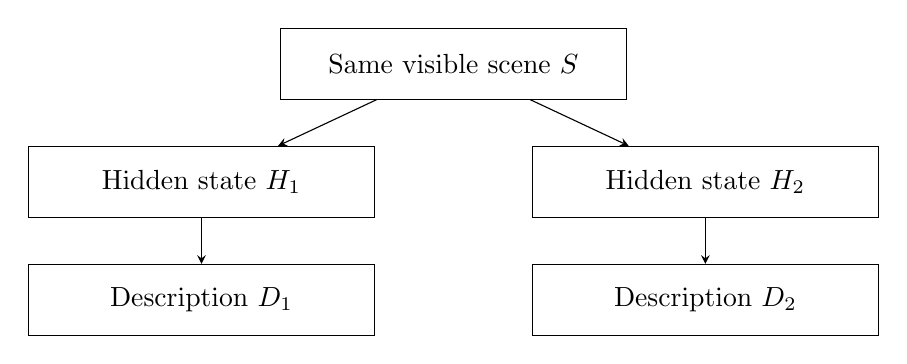
\begin{tikzpicture}[>=stealth]
\node[draw, rectangle, minimum width=4.4cm, minimum height=0.9cm] (s) at (0,2.0) {Same visible scene $S$};
\node[draw, rectangle, minimum width=4.4cm, minimum height=0.9cm] (h1) at (-3.2,0.5) {Hidden state $H_1$};
\node[draw, rectangle, minimum width=4.4cm, minimum height=0.9cm] (h2) at (3.2,0.5) {Hidden state $H_2$};
\node[draw, rectangle, minimum width=4.4cm, minimum height=0.9cm] (d1) at (-3.2,-1.0) {Description $D_1$};
\node[draw, rectangle, minimum width=4.4cm, minimum height=0.9cm] (d2) at (3.2,-1.0) {Description $D_2$};
\draw[->] (s) -- (h1);
\draw[->] (s) -- (h2);
\draw[->] (h1) -- (d1);
\draw[->] (h2) -- (d2);
\end{tikzpicture}
\caption{Transcript-based schematic reconstruction of the kitchen scene. The external setup can remain fixed while the mother's hidden history changes the language, tone, and pace of the scene.}
\end{figure}

Towles's point is subtler still. The child may not consciously know what has happened. Yet the mother's behavior must carry the trace of that hidden state, so that later, when the truth is discovered, the reader can return and say: it was all there. The scene was already vibrating with knowledge that the focal consciousness could sense but not interpret.

The lecture's iterative logic returns here with more force. We begin by observing accurately. Then we choose words. Then we revise toward a larger truth that includes not only what is visible, but the emotional field of the household, the class setting, the regional context, and the historical moment. The scene is not merely a kitchen. It is this kitchen, in this family, under these pressures.

\subsection{Question \& Answer}

\paragraph{How do we avoid cliche and still make a scene historically specific and emotionally loaded?}

By refusing to write like a historian labeling the decade. We ask instead what this perceiver, at this age and in this situation, would actually notice. Then we allow hidden state to reshape the scene's language and tempo from underneath. Historical specificity enters through lived perception, not through a pile of expected markers.

Towles then turns this example into an ethics of drafting. The first draft, he says, is written for himself alone. He lets fascinations, digressions, vanities, and odd pleasures proliferate without restraint. Only later does he reverse the lens and read from the reader's side of the covenant:
\begin{equation}
\text{first draft for self} \longrightarrow \text{revision for reader}.
\end{equation}
That second phase is not a marketing exercise. It is an obligation. If the reader is giving money and, more importantly, time, the writer owes economy in return. Redundancy, boredom, cliche, and purely private indulgence must be cut. Revision is therefore largely subtractive. It makes the prose leaner, sharper, and truer to the story's actual needs.

\section{Craft, Reading, Poetry, Manifestos, Doors, and New York}

From revision the lecture broadens into teachability. Towles refuses the posture of a formal writing teacher, but his answer is clear enough. Much can be taught if by teaching we mean repeated practice, disciplined exposure, and growing command over the elements of craft. He explicitly names a long list:
\begin{itemize}
\item plot,
\item setting,
\item dialogue,
\item tone of voice,
\item perspective,
\item metaphor,
\item simile,
\item allusion,
\item allegory.
\end{itemize}
The key word is not genius but repetition. One gains command by writing again and again, and Towles adds an important further demand: young writers should write from many points of view. Different genders, classes, ages, regions, countries, and sensibilities force the writer to rediscover craft as variable rather than fixed. There is no single formula for ``how to describe a room,'' because the room changes with the mind that enters it.

The same principle governs reading. Towles describes reading and writing as nearly simultaneous from childhood onward. He reads with a pen. He studies structure. He writes about structure. He participates in a long-running reading group that treats books comparatively and historically. The point is not passive admiration. It is investigation.

A revealing heuristic appears here. History, Towles says, is poor at preserving everything that is great, but comparatively good at discarding what is mediocre. In shorthand form:
\begin{equation}
\text{corpus at } t \longrightarrow \text{filtered canon at } t+50.
\end{equation}
We should not mistake this for a law. Towles plainly presents it as a rule of thumb. But it explains why he and his friends often read older authors: not because the past captured every greatness, but because time has already done some filtering.

Towles also lingers at the sentence level. A paragraph by Roth may move, almost invisibly, from one consciousness to another, or briefly into omniscience, without rupture. That kind of fluid viewpoint movement is powerful precisely because it is dangerous. Mishandled, it jars the reader. Handled well, it enlarges narrative possibility.

His remarks on poetry return to the problem of balance. Too much poetic indeterminacy, sustained without relief, will exhaust the reader. A novel must therefore know when to stabilize orientation and when to let language move into dream, ambiguity, or resonance. The same balance returns in his remarks on manifestos. What interests him there is not ideology as such, but verbal energy. Manifestos are declarative, staccato, confident, and action-oriented. They do not slow themselves down with too much example or exposition. In compressed form:
\begin{equation}
\text{high declaration density} + \text{low explanatory drag} \Rightarrow \text{manifesto energy}.
\end{equation}

The lecture's final metaphor gathers several of these threads at once. A promising idea is one that opens doors. The writer sees one small thing, or has one compressed premise, and immediately many rooms begin to appear. Many scenes, many directions, many layers become imaginable:
\begin{equation}
\text{premise} \Rightarrow \text{many possible continuations}.
\end{equation}
That metaphor allows the conversation to close on New York. For Towles, New York is not merely a melting pot of ethnicity or nationality. It is a melting pot of passions. Journalism, cuisine, dance, finance, law, advertising, theatre, and other pursuits all draw ambitious young people into the same urban field. The result is a density of overlapping aspiration. That density gives the city its strange electricity, and it explains why New York functions, in Towles's imagination, not only as a setting but as an engine of narrative possibility.

\subsection{Question \& Answer}

\paragraph{What makes an idea rich enough to grow into a novel rather than remain a passing observation?}

Towles's test is not abstract difficulty but branching power. A good premise begins opening rooms almost immediately. If one idea quickly suggests many scenes, many pressures, many characters, and many routes forward, then the writer feels its richness before he has fully written any of it down.

\section{Summary}

This lecture contains no literal board mathematics, yet it is rigorous in a different and very useful way. It gives us a chain of necessities. Vocabulary must belong to a world. Description must create presence. Presence must support engagement. Editing must distinguish urgency from mere speed. Planning must reduce analytic burden so that surprise can occur inside the sentence. Point of view must generate meaningful detail from within consciousness. Revision must convert private abundance into readerly economy. And reading, finally, must become a reciprocal apprenticeship in which structure, tone, sentence movement, and historical judgment continually return to the writer's own practice.

If we keep the lecture's order in mind, the whole discussion hangs together. Towles begins with language, narrows to presence, widens to process, drills down into point of view and scene construction, turns toward revision and teachability, and then opens outward again into reading, poetry, rhetorical energy, door-opening premises, and the strange urban field of New York. The result is not a doctrine of inspiration. It is a disciplined account of how imaginative freedom is built.